\chapter{Incoherent Sensing Matrix Design}
\label{chap:chap3}
%
\section{Introduction}
Compressed sensing has generated a lot of research interest in the signal and image processing communities since its introduction~\cite{Donoho, TaoNear, Taocandes}. It has gained popularity due to its ability to recover a high-dimensional signal from significantly fewer measurements than the number of ambient signal measurements required in conventional schemes. Compressed sensing allows us to exploit the sparse structure of the signal or the underlying phenomena for capturing incoherent measurements using a sensing (or projection) matrix~\cite{Elad}. In most compressed sensing applications, random sensing matrices have been used to extract significant information from the signal of interest. However, it has been shown that optimizing the sensing matrix can greatly improve the sparse signal reconstruction performance. An incoherent sensing matrix can greatly reduce the recovery error for sparse signal reconstruction. With this motivation, in this chapter, we introduce an algorithm for the construction of an incoherent sensing matrix with respect to the designed equiangular tight frame for reducing pairwise mutual coherence. The designed frame consists of a set of column vectors in a finite-dimensional Hilbert space with the desired norm and reduced pairwise mutual coherence. 

As discussed earlier, CS provides the mathematical framework for reconstructing a signal $\bm{x} \in \Re^{N \times 1}$ from linear measurements $\bm{y} \in \Re^{M \times 1}$ acquired through a sensing matrix $\bm{\Phi} \in \Re^{M \times N}$~\cite{RichardCS}:
%
\begin{align}
\label{eq:projection_2}
     \bm{y} = \bm{\Phi}\bm{x}
\end{align}
%
Traditionally, the number of measurements $M$, must be at least as large as the length of the underlying signal. This concept is related to the Nyquist-Shannon sampling theorem as discussed in Chapter~\ref{chap:intro}. However, CS allows recovery of signals of length $N$ with the number of measurements being much smaller than $N$. Further, we can reconstruct the signal $\bm{x}$ from the measurement $\bm{y}$ assuming the relation in~\eqref{eq:projection_2} with $M \ll N$. 

From Chapter~\ref{chap:intro}, we can deduce that with an optimized incoherent sensing matrix, signal recovery performance from under-sampled measurements can be greatly improved~\cite{Elad} as the reconstruction performance of CS-based system is highly dependent on the type of sensing matrix and the performance of the learned sparsifying dictionary. For reconstruction, CS relies on properties such as the spark (smallest number of linearly dependent columns) and incoherence between the columns of the dictionary $\bm{D} = \bm{\Phi}\bm{\Psi}$. As discussed earlier, computing spark is a computationally intensive task and hence CS systems rely on sensing matrix design based on incoherence. CS recovery condition requires low coherence between the sensing matrix and the transform basis matrix, such that every measurement provides new information that is not already represented by the transform basis. 

In this chapter, we focus on designing incoherent sensing matrix for improved recovery performance in CS systems. As discussed in Sections~\ref{sec: chap1_hypothesis} and~\ref{sec: Chap2_Mot_obj}, the objective of the first framework in this thesis is to optimize an incoherent sensing matrix with respect to the frame matrix. The proposed method is based on updating ETF with inertial force and constructing incoherent frame and sensing matrix using alternating minimization. The reduced mutual coherence is achieved by designing equiangular tight frame for the corresponding Gram matrix and updating the frame. The matrices are updated iteratively through the target ETF using the weighted distance between the previous iterations as inertial force. Numerical experiments were performed to evaluate the recovery performance of the proposed algorithm and the results demonstrate that our method has a better overall performance compared to the state-of-the-art sensing matrix design algorithms.
%
\section{Problem Statement}
%
An incoherent frame $\bm{D}$ is designed with respect to the updated ETF in each iteration for the given or learned sparsifying basis $\bm{\Psi}$, which is similar to minimizing the off-diagonal elements of the Gram matrix $\bm{G}$. Hence, the cost function for sensing matrix design~\eqref{eq:cost_func} aims to reduce the mutual coherence by designing an ETF and then updating the $\bm{D}$ and $\bm{\Phi}$ at each iteration based on the designed ETF.
%
\begin{align}
 \label{eq:cost_func}
    \|\bm{D}^{T}\bm{D}-\bm{I}\|_{F}^{2} = \|\bm{\Psi}^{T}\bm{\Phi}^{T}\bm{\Phi}\bm{\Psi}-\bm{I}\|_{F}^{2}   
\end{align}
%
In this chapter, the Gram matrix $\bm{G} = \bm{D}^{T} \bm{D}$ is not optimized directly with respect to the identity matrix but with a designed ETF at each iteration. Here, the updated $\bm{G}$ will be close to the corresponding ETF designed by the algorithm and contained within the convex set $H_{\mu}$:
%
\begin{align}\nonumber
    H_{\mu} \triangleq \{\bm{H} \in \Re^{L \times L}: \bm{H}=\bm{H}^{T}, \bm{H}_{ii}=1, \underset{i\neq j}{\max}\lvert \bm{H}_{ij}\rvert \leq \mu_{W}\}
\end{align}
%
For designing an incoherent frame $\bm{D}$, cost function in~\eqref{eq:cost_func} is reformulated and posed as the following minimization:
%
\begin{align}
    \label{eq:frame_D_opt}
    \underset{\bm{D}}{\min} \quad \|\bm{E}\|_{F}^{2} + P_{\Pi}(\bm{D}) \quad \text{s.t.} \quad \bm{E} = \bm{D}^{T}\bm{D}-\bm{H}
\end{align}
%
where $\bm{H} \in H_{\mu}$, and $P_{\Pi}(\bm{D})$ defines the projection of $\bm{D}$ onto a convex set $\Pi$ which regulates its column norm, given by:
%
\begin{equation}\nonumber
    P_{\Pi}(\bm{D}): \{\bm{d_{i}}\}_{i=1}^{L} =
    \begin{cases}
      \bm{d_{i}} & \quad \|\bm{d_{i}}\|_{2} < 1\\
      \frac{\bm{d_{i}}}{\|\bm{d_{i}}\|_{2} } & \quad \text{otherwise}.\\
    \end{cases} 
\end{equation}
%
For updating the ETF $\bm{H}$, we reduce the larger off-diagonal elements by projecting $\bm{G}$ onto $H_{\mu}$ at each iteration and then updating $\bm{D}$. We use $\mu_{W}$ as the threshold for updating $\bm{H}$. Let $\bm{E_{p}} = \bm{D_{k}}^{T} \bm{D_{k}}-\bm{I}$ at the $p^\text{th}$ outer iteration, then after projecting $\bm{E}$ onto $H_{\mu}$ we obtain the ETF. This is achieved by constraining the off-diagonal elements of $\bm{E}$ using the shrinkage function $S_{\Omega_{\mu}}$.
%
\begin{equation}
    \label{eq:shrinkage_fn}
    S_{\Omega_{\mu}}(\bm{E}): \underset{(i\neq j)}{\bm{E}_{ij}} =
    \begin{cases}
      \bm{E}_{ij} & \lvert \bm{E}{ij}\rvert \leq \mu_{W} \\
      \text{sign}(\bm{E}_{ij})\cdot\mu_{W} & \quad \text{otherwise}
    \end{cases}
\end{equation}
%
At each iteration this ensures that the large off-diagonal elements will be reduced in magnitude. Unlike other algorithms which project $\bm{E}$ onto the set of ETF via a shrinkage function, here we apply shrinkage on the weighted difference of the off-diagonal elements which is an estimate of the distance between the updated $\bm{E}$ and the corresponding ETF. The update scheme can be accelerated by incorporating an inertial force. The inertial force is computed as the weighted difference of the estimates of $\bm{E}$ from iterations $p$ and $(p-1)$.
%
\begin{align}
    \label{eq:EH_inertial_force}
    & \bm{E}_{p} = \bm{D}_{k}^{T}\bm{D}_{k} - \bm{I}\nonumber\\ 
    & \bm{H}_{p} = \bm{E}_{p} + w_{1}(\bm{E}_{p} - \bm{E}_{p-1})
\end{align} 
%
where $w_{1} \geq 0$ is a weighting parameter. At each iteration, $\bm{E_{p}}$ is computed using the current distance between the Gram matrix and ETF along with the inertial force. 
%
\begin{equation}
    \label{eq:H_update}
    \bm{H}_{p+1} = S_{\Omega_{\mu}}(\bm{H}_{p}) + \bm{I} 
\end{equation}
%
%It adds the weighted quantity of the distance between the two respective iterations indicating if it's converging.
%
\subsection{Incoherent Frame Design}
%
For updating $\bm{D}$ and $\bm{\Phi}$, we apply the alternating minimization method to the updated $H$.  In~\cite{Frame}, authors have shown different methods for designing incoherent sensing matrix corresponding to an ETF using alternating minimization. At each iteration, $\bm{D}$ is updated corresponding to the ETF $\bm{H}$ via the gradient method with inertial force. Let us denote the objective function for $\bm{D}$ %in~\eqref{eq:frame_D_opt} 
by $J =  \underset{\bm{D}}{\min}\|\bm{D'D -H}\|_{F}^{2} $  and the derivative of $J$ with respect to $\bm{D}$ as $\nabla_{\bm{D}}(J)$:
%
\begin{align}\nonumber
    %\label{eq:J_derivative}
    \nabla_{\bm{D}}(J) = 4\bm{D}\left(\bm{D}^{T}\bm{D} - \bm{H}\right)
\end{align}
%
\begin{equation}
    \label{eq:D_update}
     \bm{D}_{k + 1} = \bm{D}_{k} - \eta\bm{D}_{k}\left(\bm{D}_{k}^{T}\bm{D}_{k} - \bm{H}_{p+1}\right)
\end{equation}
%
Similar to~\eqref{eq:EH_inertial_force}, the update step for $\bm{D}$ in~\eqref{eq:D_update} can be modified to use an inertial force by taking a weighted difference of the estimates of $\bm{D}$ from iterations $k$ and $(k-1)$:
%
\begin{align}
    \bm{D}_{k + 1/2} = \bm{D}_{k} - \eta\bm{D}_{k}\left(\bm{D}_{k}^{T}\bm{D}_{k} - \bm{H}_{p+1}\right)\nonumber\\
    \bm{D}_{k + 1} = P_{\Pi}\left(\bm{D}_{k+ 1/2}\right) + w_{2}\left(\bm{D}_{k} - \bm{D}_{k-1}\right)
\end{align}
%
where $\eta$ is the step-size and $w_{2} \geq 0$ is a weighting parameter. Using the updated $\bm{D}$, we update $\bm{\Phi}$ by solving:
%
\begin{equation}
    \label{eq:Phi_update}
    \bm{\Phi}_{k + 1} = \underset{\bm{\Phi}}{\min} \|\bm{D}_{k+1} - \bm{\Phi \Psi}\|_{F}^{2}
\end{equation}
%
In each iteration, the algorithm alternately updates $\bm{H}_{p+1}$ using~\eqref{eq:H_update} followed by updating $\bm{D}_{k + 1}$ and $\bm{\Phi}_{k+1}$ using~\eqref{eq:D_update} and~\eqref{eq:Phi_update}, respectively. The alternating minimization iterations are repeated until convergence is achieved.
%i.e., $\| \bm{\Phi}_{k+1} - \bm{\Phi}_{k} \|_{F}^{2}$ is less than a threshold, or when the maximum number of iterations is reached. Note that we set the stopping threshold to $0.01$ in the ISMD method. 
In addition, alternating minimization does not increase the distance between successive iterations~\cite{Frame}~\cite{Lewis_convergence}. However, the convergence proof of alternating minimization does not hold when the constraint sets are non-convex which is still an open problem. Hence, in Section~\ref{sec: Chap3_results}, we discuss convergence of the ISMD algorithm based on the evolution of mutual coherence. The sensing matrix design algorithm is summarized in Algorithm 1.
%
\begin{algorithm}
\SetAlgoLined
\textbf{Objective}: Design incoherent sensing matrix.\\
\textbf{Input}: Sparsifying basis $\bm{\Psi}$, weighting parameters $w_{1}$, $w_{2}$, step size $\eta$, number of iterations $N_{total}$, $N_{outer}$, and $N_{inner}$.\\
 \textbf{Initialization}: Initialize $\bm{\Phi}$ to a random matrix.\\
 \While{$i < N_{total}$}{
  \For{$p = 1:N_{outer}$}{ 
  Update ETF $\bm{H_{p+1}}$ using~\eqref{eq:H_update}\\
  \For{$k = 1:N_{inner}$}{
   Update $\bm{D_{k+1}}$ using~\eqref{eq:D_update}\\
   Update $\bm{\Phi_{k+1}}$ using~\eqref{eq:Phi_update}}
   $\bm{\Phi_{k+1}} = \bm{\Phi_{N_{inner}}}$} 
   $i = i + 1$}
 \textbf{Output}: Sensing matrix $\bm{\Phi_{output}}$
 \caption{Incoherent sensing matrix design (ISMD) using alternating minimization}
\end{algorithm}
%

In the proposed incoherent sensing matrix design algorithm, shrinkage function $S_{\Omega_{\mu}}$ is applied only on the off-diagonal elements and updated with an inertial force. Diagonal elements of $\bm{H}$ remain unity during the update step~\eqref{eq:H_update} due to which a normalization step is not required. Step size $\eta$ and weighting parameters $w_{1}$ and $w_{2}$ are determined empirically. With $w_{1}=w_{2}=0.80$ incoherent frames were obtained and a step-size $\eta = 0.09$ is used to avoid divergence. For updating $\Phi$, $N_{inner} = 3$ gives good results. The update process is repeated $100$ times i.e., $N_{total} = 100$. However, other stopping criteria can also be used. For example, the algorithm may iterate until the $\| \bm{\Phi}_{k+1} - \bm{\Phi}_{k} \|_{F}^{2}$ is less than a certain threshold, or until $\bm{D}$ achieves a predefined coherence threshold. For the proposed ISMD algorithm, we assume convergence is achieved when either $\| \bm{\Phi}_{k+1} - \bm{\Phi}_{k} \|_{F}^{2}$ is less than $0.01$, or the maximum number of iterations is reached. 
%
%%============================================================%%
\section{Experimental Results}
\label{sec: Chap3_results}
%
In this section, we illustrate the performance of the proposed ISMD algorithm and compare it with some of the key sensing matrix design methods from literature including random Gaussian matrix, $\text{CS}_\text{Elad}$~\cite{Elad}, method in~\cite{Zelnik} referred to as "Zelnik-Manor-Rosenblum-Eldar" ($\text{CS}_\text{ZMRE}$), gradient descent based algorithm in~\cite{Vahid} referred to as "Abolghasemi-Ferdowsi-Sanei" ($\text{CS}_\text{AFS}$), and method in~\cite{Sapiro} referred to as "Duarte-Carvajalino-Sapiro" ($\text{CS}_\text{DCS}$). We use the author-provided source codes for all the algorithms, except $\text{CS}_\text{AFS}$ which we have implemented. We compare these methods via extensive numerical experiments for $100$ runs each. For ISMD, we set $N_{outer} = 15$. The algorithm parameters are kept fixed across the entire set of experiments. The initialized random matrix is generated for $N=80$, $L=100$, $M=25$ with sparsity level $s=15$. For Elad's algorithm, the other parameters are: $t= 0.4$ and $\gamma = 0.95$. In Fig.~\ref{Histogram Figure}, histogram of the absolute correlation between atoms of the frame is presented. It illustrates the distribution of the absolute off-diagonal values of the normalized Gram matrix for each algorithm. It is noted that the histogram for the ISMD algorithm displays a shift towards the left (or origin), which indicates reduction in the pairwise correlation.

%%%%%%%%%%%%%%%%%%%% Histogram %%%%%%%%%%%%%%%%%%%%%%%%%
\begin{figure}
\centering
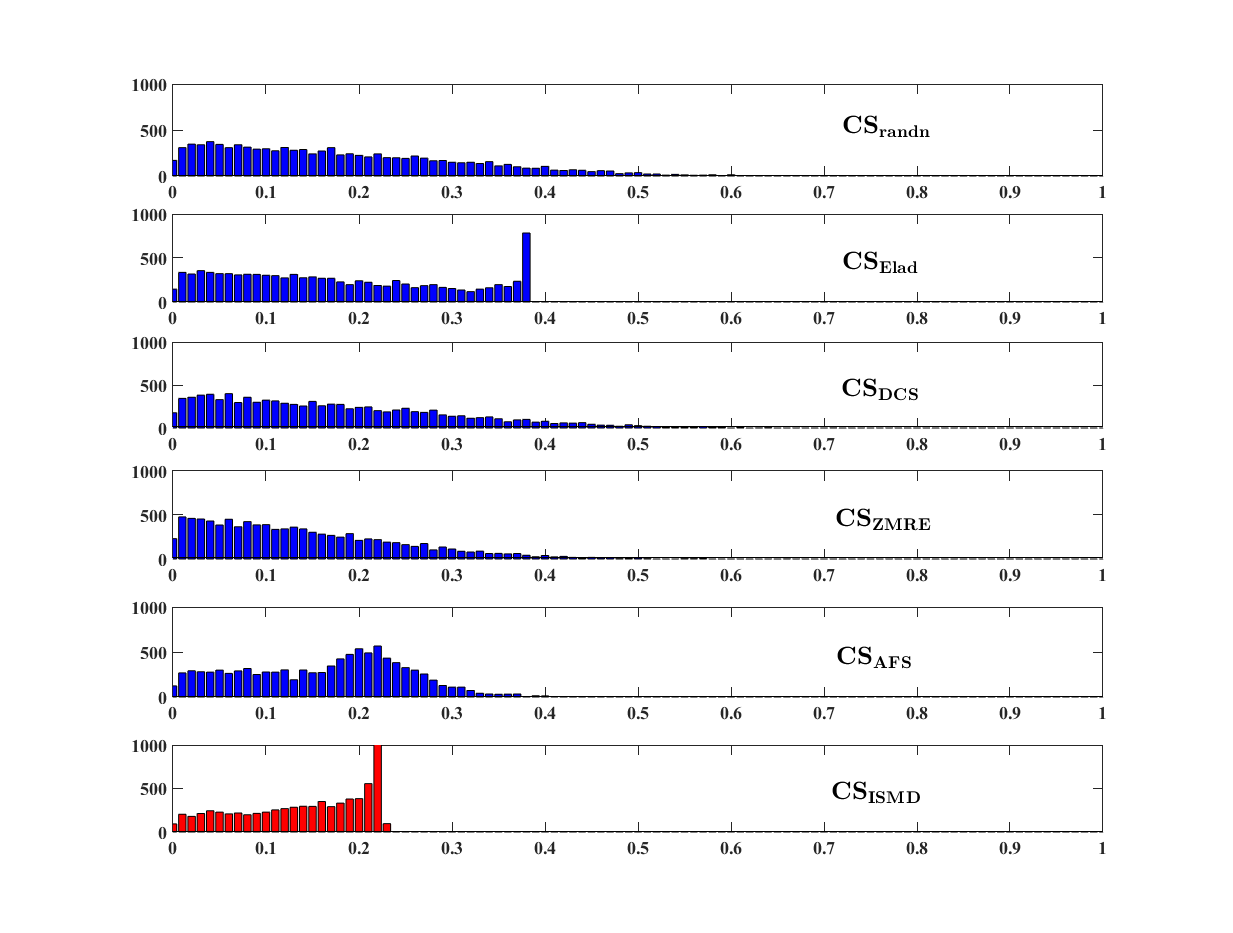
\includegraphics[keepaspectratio,width=0.8\textwidth,trim=50 20 50 20,clip]{figChap3/Hist_final.eps}
\caption{Histogram of the absolute off-diagonal values of the optimized Gram matrix ($N=80$, $L=100$, and $M=25$).}
\label{Histogram Figure}
\end{figure}
%%%%%%%%%%%%%%%%% Evolution of coherence %%%%%%%%%%%%%%%%% 
\begin{figure}
\centering    
\subfigure[Evolution of $t$-averaged mutual coherence ($\mu_{t}$)]{\label{fig:mu_t}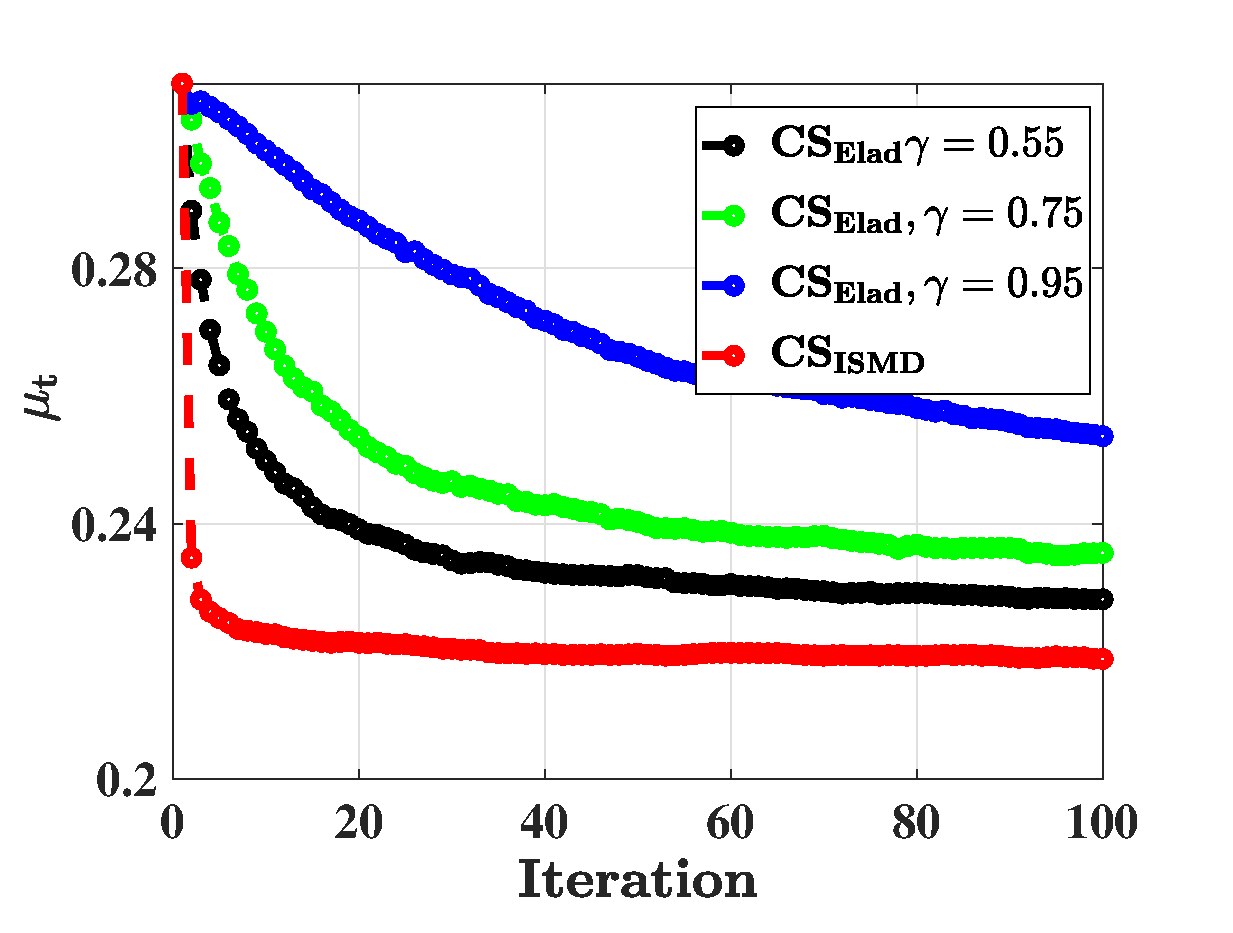
\includegraphics[keepaspectratio,width=0.45\textwidth,trim=0 0 40 2,clip]{figChap3/Coherence_final.eps}} 
\subfigure[Evolution of cumulative coherence]{\label{fig:cum_coh}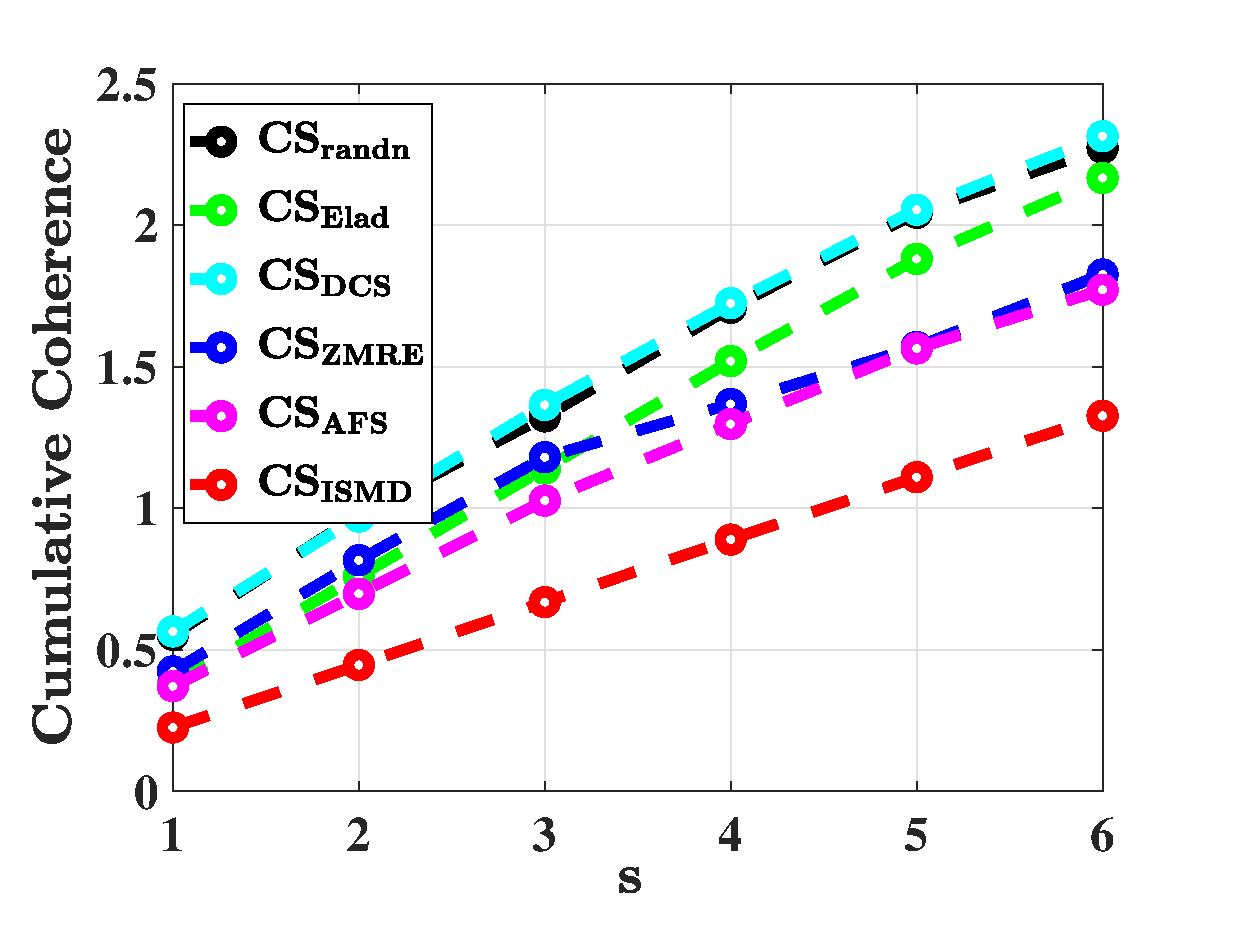
\includegraphics[keepaspectratio,width=0.45\textwidth,trim=0 10 40 2,clip]{figChap3/Babel_final.eps}}
\caption{Evolution of coherence parameters for $N=80$, $L=100$, $M=25$, and $t=\mu_{W}=0.4$, for $100$ trials. Note that for cumulative coherence, $m$ is taken as sparsity $s$ (refer~\eqref{eq: Cum_coherence} in Chapter~\ref{chap:intro}).}
\label{Fig Coherence}
\end{figure}
%%============================================================%%

Next, we consider the averaged mutual coherence $\mu_{t}$ and cumulative coherence as performance metrics since these are better measures of average recovery performance than the mutual coherence $\mu$. Cumulative coherence measures the maximum total mutual coherence between a fixed set of atoms and a collection of other atoms in the dictionary.
%
The evolution of these two performance parameters is shown in Fig.~\ref{Fig Coherence}. It is seen that the proposed ISMD algorithm results in significantly smaller values for $\mu_{t}$ and cumulative coherence. In Fig.~\ref{Fig Coherence}, the cumulative coherence of the optimized sensing matrix using ISMD is better than the other algorithms, especially $\text{CS}_\text{randn}$, $\text{CS}_\text{Elad}$, and $\text{CS}_\text{DCS}$ algorithms. We note that cumulative coherence of all the algorithms increases approximately linearly with the signal sparsity level $s$. As discussed in Section~\ref{sec: Chap_1_intro_CS}, it is seen that ISMD shows superiority in terms of the coherence measures.

%%%%%%%%%%%%%%%%%% Recovery Error %%%%%%%%%%%%%%%%%%%%%%%%%%%
\begin{figure}
\centering    
\subfigure[]{\label{fig:MSE_K}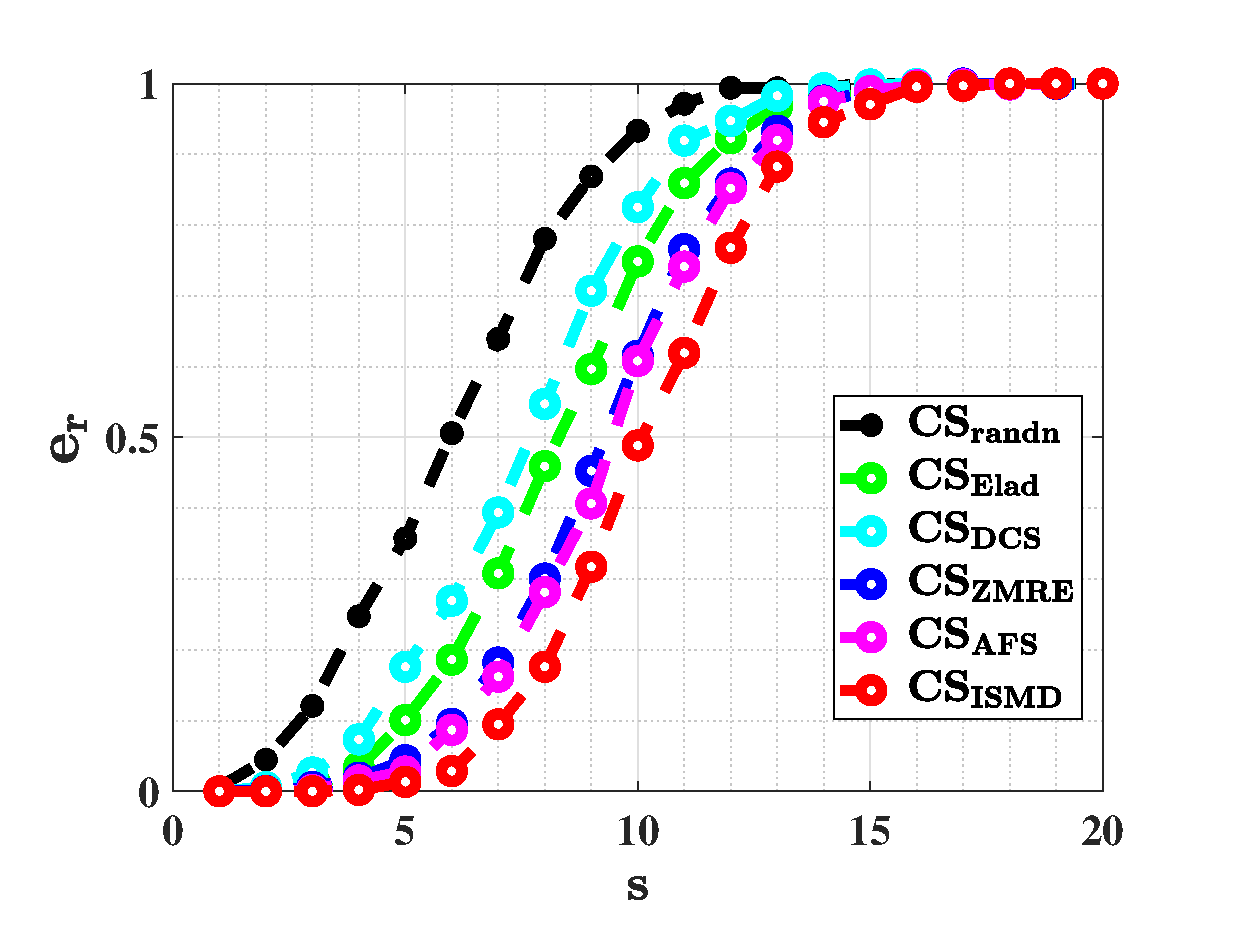
\includegraphics[keepaspectratio,width=0.45\textwidth,trim=0 5 40 25,clip]{figChap3/Recovery_final.eps}} 
\subfigure[]{\label{fig:MSE_M}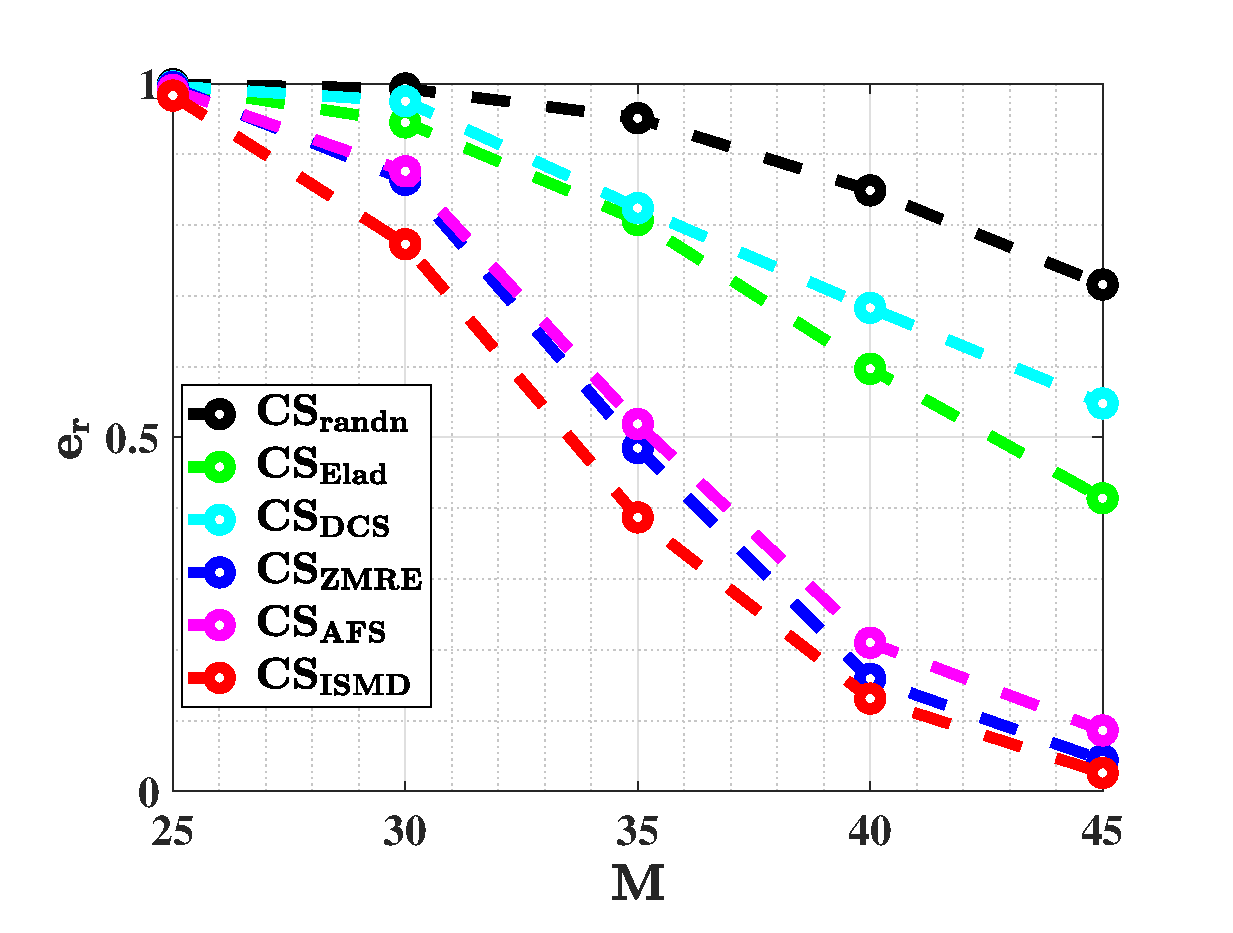
\includegraphics[keepaspectratio,width=0.45\textwidth,trim=0 5 40 25,clip]{figChap3/M_final.eps}}
\caption{Recovery performance error $e_{r}$ along varying sparsity $s$ and varying number of measurements $M$ for $N=80, L=100, M=25$ with optimized sensing matrix}
\label{Recovery results with sparsity and M}
\end{figure}
%%%%%%%%%%%%%%%%%%%%%%%%%%%%%%%%%%%%%%%%%%%%%%%%%%%%%%%%%%%%%
As seen in Table~\ref{table: ISMD_table_example}, $\text{CS}_{\text{ISMD}}$ has the least averaged mutual coherence but $\lVert I - G\rVert_{F}$ is comparable to $\text{CS}_\text{ZMRE}$. However, ISMD yields improved performance in terms of the signal reconstruction accuracy. For evaluating the recovery performance we performed two sets of experiments. Using a learned or given transform basis $\bm{\Psi}$, we generate a set of $N_{\textrm{s}}=1500$ signals with $\theta_{j}$ ($j=1,\dots,N_{\textrm{s}}$) which are $K$-sparse. Measurement vectors $\bm{y}_{j}$ are computed for these signals using $\bm{\Phi}$ designed by the above mentioned algorithms with a fixed sparsifying basis $\bm{\Psi}$. OMP algorithm is used for recovering the sparse vectors from the measurements using~\eqref{eq:L0_reconstruction}. The average reconstruction error is computed as:
%
\begin{equation}
\label{eq 23}
e_{r} = \frac{1}{N_{\textrm{s}}} \sum_{j=1}^{N_{\textrm{s}}} \frac{\|x_{j}-\widehat{x_{j}}\|_{2}^{2}}{\|x_{j}\|_{2}^{2}} 
\end{equation}
%
where $\widehat{x_{j}}$ is the recovered sparse signal. We first study the reconstruction performance with the number of iterations. Fig.~\ref{Recovery results with sparsity and M} shows that as the signal becomes less sparse (higher $K$), the reconstruction error increases gradually.

Next, we study the reconstruction performance as a function of the number of measurements. In Fig.~\ref{Recovery results with sparsity and M}, we see that the recovery performance improves as the number of measurements ($M$) increases. Fig.~\ref{Recovery results with sparsity and M} illustrates the improvement in recovery performance when using an optimized sensing matrix $\bm{\Phi}$ using the ISMD algorithm. In addition, the performance of the proposed ISMD algorithm is consistently better compared to the other methods when using OMP algorithm for reconstruction. Algorithms such as OMP used for sparse reconstruction rely on the orthogonality of the columns of $\bm{D}$ and the ISMD algorithm achieves this to a greater extent than the other methods.
%
\begin{table}
\renewcommand{\arraystretch}{1}
\caption{Performance evaluation of various CS systems (M = 25, N = 80, L = 100 AND SNR = 20 dB)}
\label{table: ISMD_table_example}
\centering
\begin{tabular}{|c|c|c|}
\hline
\bfseries  & \bfseries $|| I - G ||_{F}^{2} \times 10^{5}$ & \bfseries $\mu_{t}$  \\
\hline
$\text{CS}_{\text{randn}}$ & 4.465 & 0.3038\\
\hline
$\text{CS}_{\text{Elad}}$ & 0.00473 & 0.2875 \\
\hline
$\text{CS}_{\text{DCS}}$ & 0.00492 & 0.2961 \\
\hline
$\text{CS}_{\text{ZMRE}} $ & 0.00301 & 0.2647 \\
\hline
$\text{CS}_{\text{AFS}}$ & 0.00341 & 0.2339 \\
\hline
$\text{CS}_{\text{ISMD}}$ & 0.00307 & 0.2126 \\
\hline
\end{tabular}
\end{table}
%
\section{Chapter Summary}
%
In this chapter, we presented a framework for the design of an incoherent sensing matrix for CS applications. The proposed ISMD algorithm was shown to design an optimized sensing matrix whose columns have reduced mutual coherence as per the hypothesis discussed in Section~\ref{sec: chap1_hypothesis}. The optimized sensing matrix can achieve improved recovery performance with reduced mutual coherence. We design an ETF using inertial force update and the corresponding frame and sensing matrix are updated using the alternating minimization method. The designed sensing matrix was also shown to have reduced cumulative coherence. The proposed method achieves improved recovery performance (or achieves the same recovery performance with fewer measurements) as the state-of-the-art algorithms in the literature. The experiments have illustrated that the proposed method outperforms the other methods in recovery performance.